\documentclass[11pt,a4paper]{article}
\title{Reservoir Simulation, Exercise 1}
\author{Einar Baumann}

\usepackage[T1]{fontenc}
\usepackage{droid}
\usepackage[defaultsans]{opensans}
\usepackage{bera}
\usepackage{listings}
\usepackage{float}
\usepackage{graphicx}
\usepackage{booktabs} 
\usepackage{subfig}  

\usepackage{caption}
\captionsetup{margin=10pt,font=small,labelfont=bf}

\usepackage{sectsty}
\allsectionsfont{\normalfont\sffamily}

\usepackage{color}
\definecolor{light-gray}{RGB}{250,250,250}  % Background color for listings
\definecolor{gray}{RGB}{100,100,100}  % Color for line-numbers
\lstset{
  language={C},     % the language of the code
  aboveskip=0em,
  belowskip=3em,
  basicstyle=\ttfamily\scriptsize,
  backgroundcolor=\color{light-gray},
  frame=single,       % adds a frame around the code
  rulecolor=\color{black},  % frame color
  captionpos=t,       % sets the caption-position to bottom
  breaklines=true,      % sets automatic line breaking
  breakatwhitespace=false,  % automatic breaks only at whitespace?
  keepspaces=true,      % keeps spaces in text, useful for keeping indentation of code (possibly needs columns=flexible)
  tabsize=4,          % sets default tabsize to 2 spaces
  commentstyle=\color{green}, % comment style
  keywordstyle=\color{blue},  % keyword style
  stringstyle=\color{red},  % string literal style
  numbers=left,       % line-number position: none, left or right
  numbersep=5pt,        % how far the line-numbers are from the code
  numberstyle=\tiny\color{gray}, % the style that used for line-numbers
  stepnumber=2,       % step between two line-numbers.
  showspaces=false,     % show spaces everywhere with underscores
  showtabs=false,       % show tabs within strings with underscores
  showstringspaces=false,   % underline spaces within strings only
  escapeinside={\%*}{*)},   % if you want to add LaTeX within your code
  title=\lstname        % show the filename of files included with \lstinputlisting; also try caption instead of title
}


\begin{document}
\maketitle

\section{Derivations} % (fold)
\label{sec:derivations}
this is a test. \texttt{monospace test}

% section derivations (end)

\pagebreak


\section{FORTRAN program} % (fold)
\label{sec:fortran_program}

\subsection{Plots} % (fold)
\label{sub:plots}

\begin{figure}[H]
  \centering
  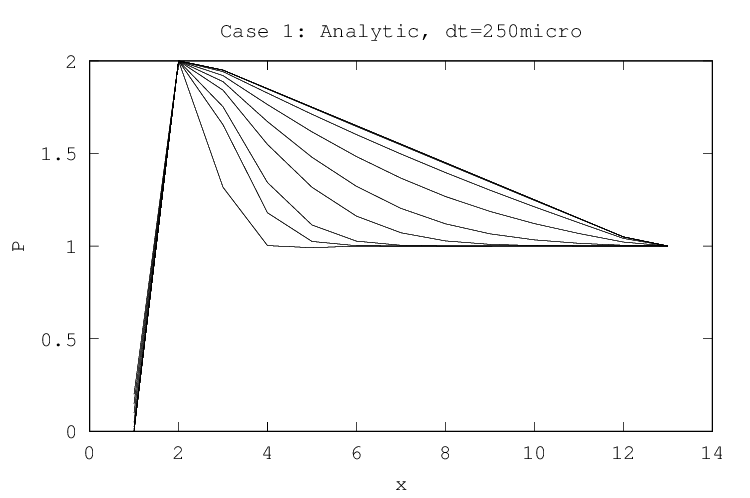
\includegraphics[]{../code/case1.png}
  \caption{Case 1.}
  \label{fig:case1}
\end{figure}

\begin{figure}[H]
  \centering
  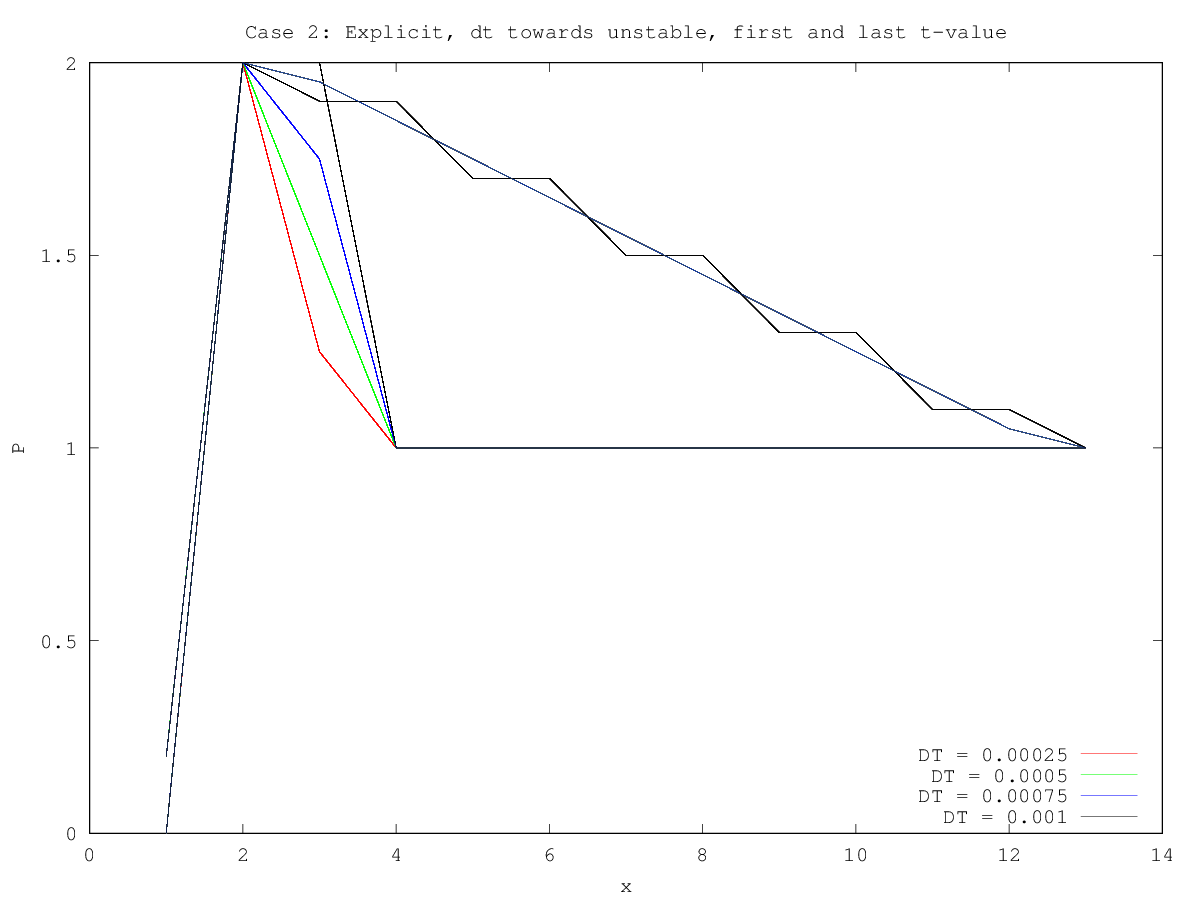
\includegraphics[]{../code/case2.png}
  \caption{Case 2.}
  \label{fig:case2}
\end{figure}

\begin{figure}[H]
  \centering
  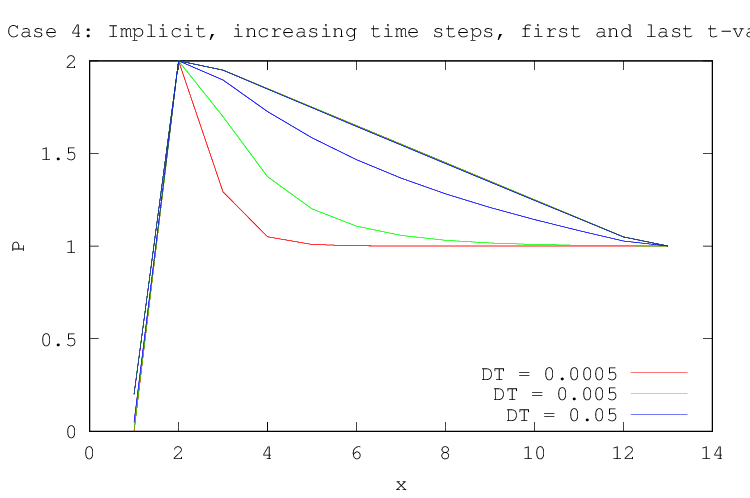
\includegraphics[]{../code/case4.png}
  \caption{Case 4.}
  \label{fig:case4}
\end{figure}

\begin{figure}[H]
  \centering
  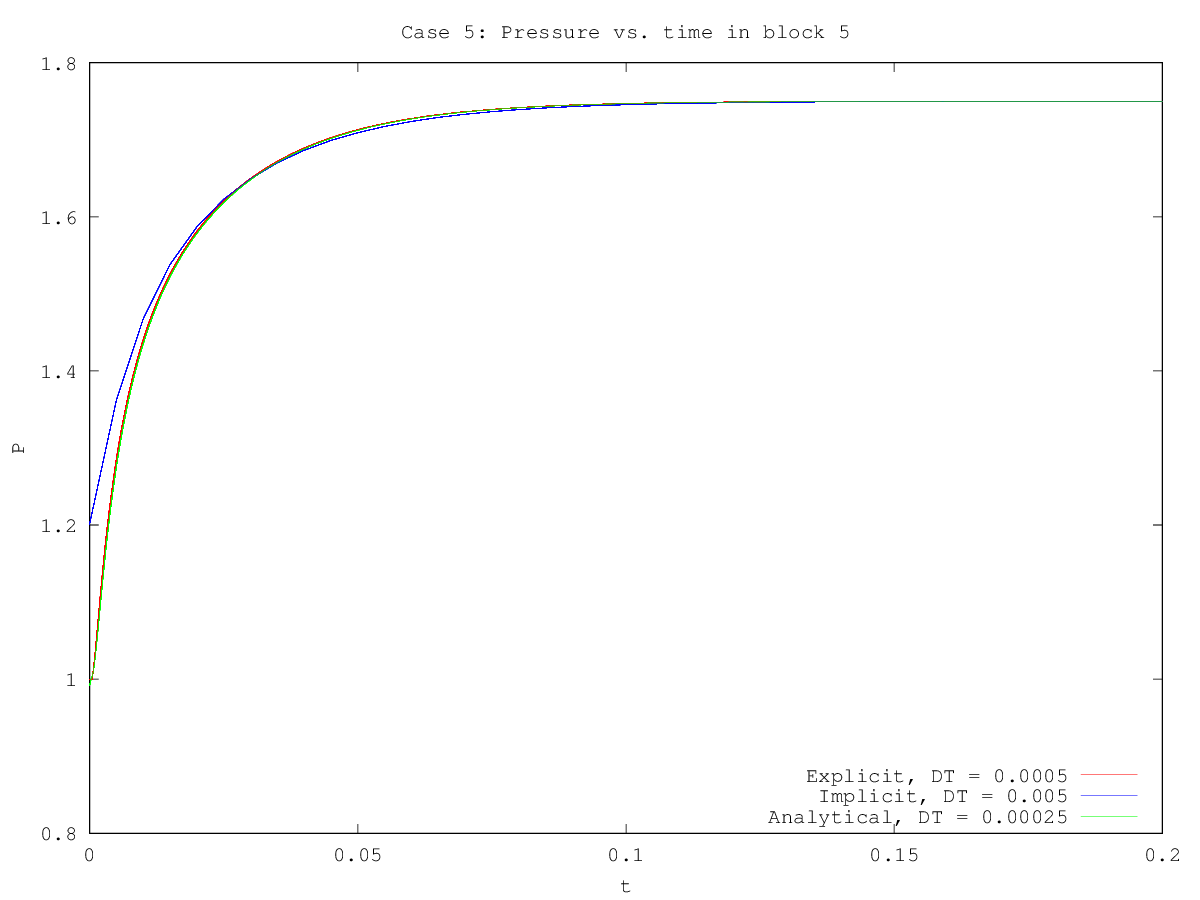
\includegraphics[]{../code/case5.png}
  \caption{Case 5.}
  \label{fig:case5}
\end{figure}

\begin{figure}[H]
  \centering
  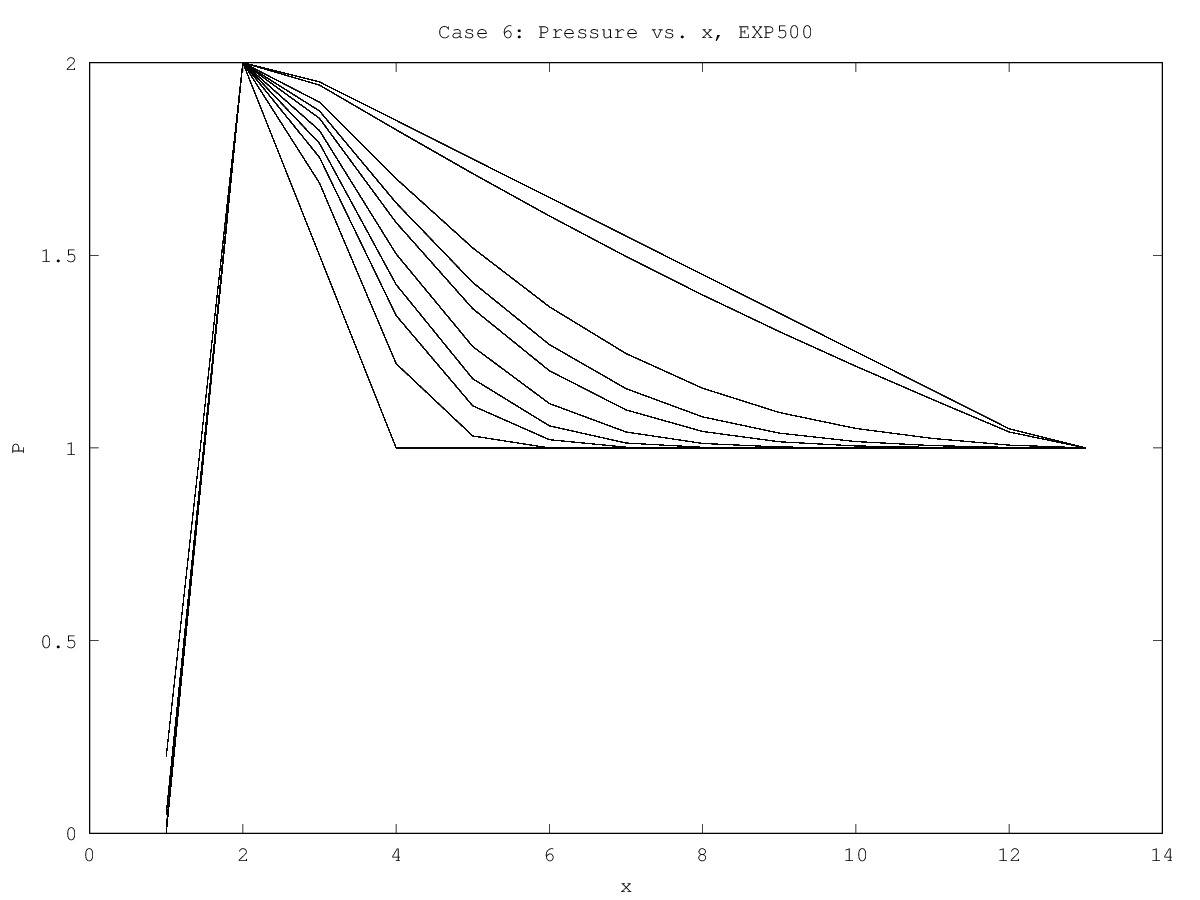
\includegraphics[]{../code/case61.png}
  \caption{Case 6, explicit solution.}
  \label{fig:case61}
\end{figure}

\begin{figure}[H]
  \centering
  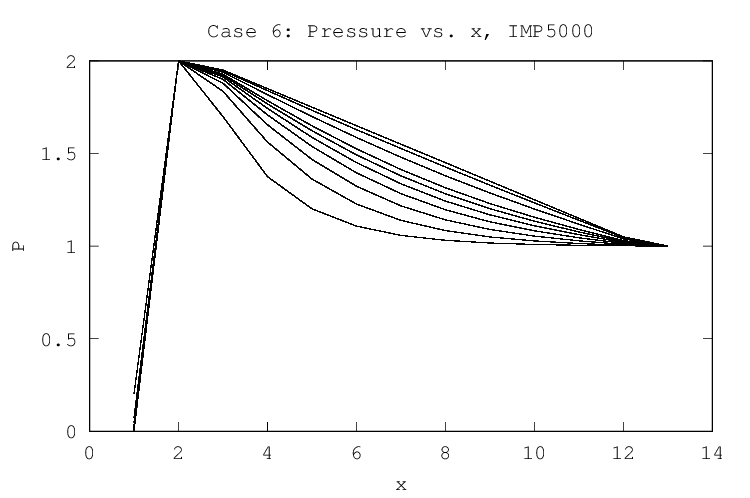
\includegraphics[]{../code/case62.png}
  \caption{Case 6, implicit solution.}
  \label{fig:case62}
\end{figure}

\begin{figure}[H]
  \centering
  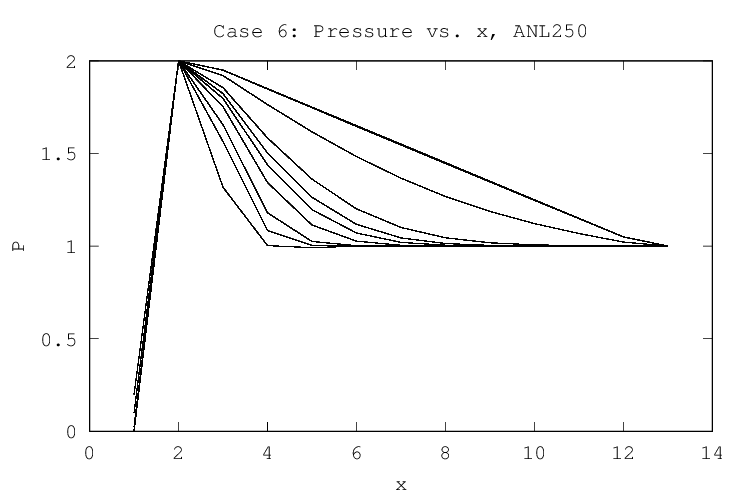
\includegraphics[]{../code/case63.png}
  \caption{Case 6, analytical solution.}
  \label{fig:case63}
\end{figure}

% subsection plots (end)
\pagebreak

\subsection{Listings} % (fold)
\label{sub:listings}

\lstinputlisting[%
  caption={Main program},
  label={lst:mainprog},
  language={[90]Fortran}]
  {../code/MainProg.f90}

\lstinputlisting[%
  caption={Shell script for data set generation},
  label={lst:shellscript},
  language={sh}]
  {../code/GenerateData.sh}

\lstinputlisting[%
  caption={Matlab script for plot generation},
  label={lst:plotgen},
  language={Matlab}]
  {../code/GeneratePlots.m}
% subsection listings (end)


% section fortran_program (end)
  
\end{document}
